% !TeX root = ../HebutThesis_example.tex(此文件是被HebutThesis_example.tex调用的)
\chapter{插图插表及引用参考文献方法(仅供参考)}

\section{插图}
插图:一般情况下,在正文中,先见到图号和图的内容再展示图。
特殊情况须延后的插图不应跨节。

通常使用的函数图采用简化形式,称为简写函数图,例如图{\ref{fig:historyhebut}}以及图{\ref{fig:河北工业大学校门}}。
% 引用图的方法:在正文中插入\ref{tab:表的名称}
\begin{figure}[ht]
    \centering                                                      % 居中
    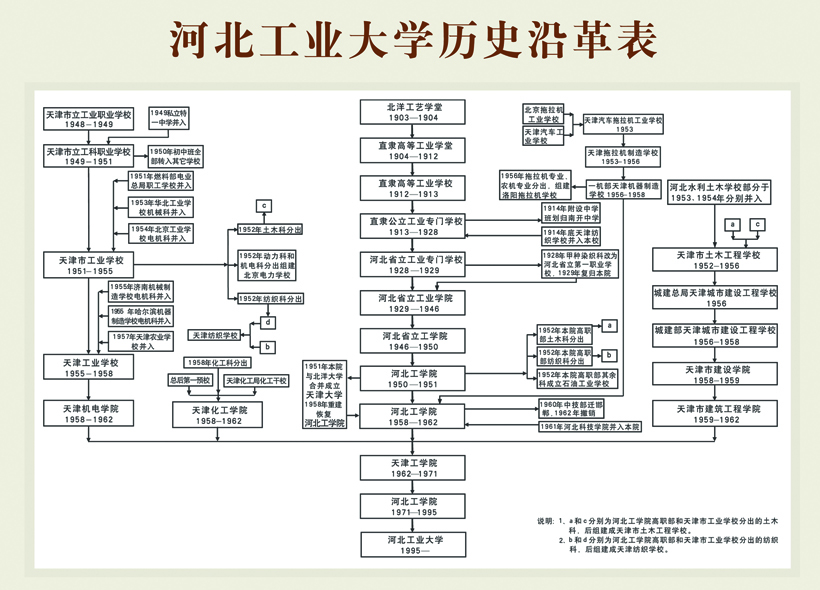
\includegraphics[width=0.5\textwidth]{figures/historyhebut}     % 页面宽度为文本宽度的0.5倍
    \caption{河北工业大学历史沿革}\label{fig:historyhebut}            % caption后为设定的图片名称,label后为图片文件名称
\end{figure}

\begin{figure}[ht]
    \centering
    
\includegraphics[width=\textwidth]{figures/河北工业大学校门}
    \caption{河北工业大学校门}\label{fig:河北工业大学校门}
\end{figure}

\section{插表}
一般情况下,表格须通栏,即表格宽度与正文版面平齐,
简单的表可以使用tabular包。如\ref{tab:table_example}所示,
复杂的可以使用tabularx包,如三线表\ref{tab:table_centered}所示。
% 引用表的方法:在正文中插入\ref{tab:表的名称}
两种包的区别:

使用tabular时,列宽基于内容或者指定的宽度,表格宽度自适应。

使用tabularx时,表格宽度固定,X格式列的宽度自动调整以适应表格总宽度。
允许指定表格的总宽度,X列会自动调整宽度,以填满指定的表格宽度。
适用于需要表格宽度匹配特定尺寸(如页面宽度)的场景。

\begin{table}[ht]
    \centering
    \caption{表格示例}
    \label{tab:table_example}
    \begin{tabular}{|l|c|r|}
    \hline
    左对齐 & 居中对齐 & 右对齐 \\ \hline
    数据1 & 数据2 & 数据3 \\
    数据4 & 数据5 & 数据6 \\ \hline
    \end{tabular}
\end{table}


\begin{table}
    \centering
    \caption{三线表示例}\label{tab:table_centered}      % caption后为设定的表格上名称,label后为表格标签
    \begin{tabularx}{\textwidth}{>{\centering\arraybackslash}X>{\centering\arraybackslash}X>{\centering\arraybackslash}X}
    % {\textwidth}用于调整表总宽度
    % >{\centering\arraybackslash}:这是列格式的预定义设置,
    % 用于使列中的内容居中。>{}用于在进入列前插入指定的命令,
    % 这里是\centering命令,用于使列中的文本居中对齐。\arraybackslash是必要的,
    % 因为\centering命令会重定义\\命令,而在表格中\\用于换行,
    % 所以需要\arraybackslash来恢复\\的原始功能,即结束当前行。
    \toprule
    列1 & 列2 & 列3 \\
    \midrule
    有效 & 001 & 通过 \\
    无效 & 002 & 未通过 \\
    文本1 & 文本2 & 长文本3的内容可能会更多,但这三列的宽度会自动平均分配。\\
    文本4 & 文本5 & 文本6 \\
    \bottomrule
    \end{tabularx}
\end{table}

\section{引用}
本文档中参考文献样式标准以GB/T 7714-2015为准,使用了 biblatex-gb7714-2015 宏包。
biblatex-gb7714-2015 宏包是为满足《GB/T 7714-2015 信息与文献 参考文献著录规则》要求而开发的 biblatex 样式包。

使用时在 bibliography.bib 文件添加文献管理工具如 Zotero、ReadPaper、Google Scholar 导出的 BibTex 格式,如

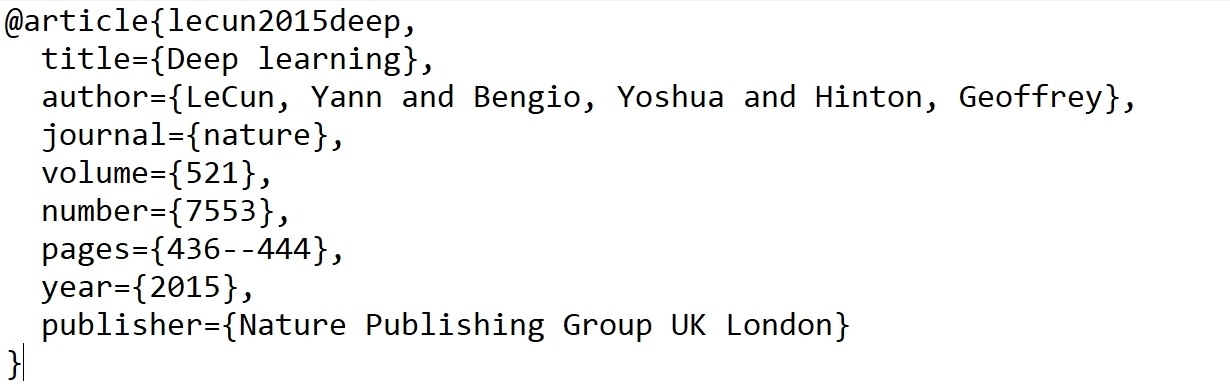
\includegraphics[width=0.5\linewidth]{figures/参考文献.png}

之后在正文部分使用{{{$\backslash$}cite}}命令可以引用\cite{lecun2015deep}。
随后,可自动在最后的参考文献部分生成参考文献列表。

